\section{Configuración del servidor FreeIPA}\label{sec:configuracion-servidor-freeipa}

Una vez finalizada la instalación del servidor, se procedió a realizar la configuración inicial de la plataforma FreeIPA, incorporando los usuarios, grupos y políticas necesarios para el funcionamiento de la infraestructura y la integración de los servicios definidos durante la fase de diseño.

\subsection{Creación de grupos de usuarios}

Una vez finalizada la instalación de la plataforma, se procedió a la creación de los grupos de usuarios necesarios para la gestión del acceso a los servicios integrados en la infraestructura. Estos grupos constituyen el principal mecanismo de autorización, ya que permiten asociar a cada usuario los permisos correspondientes en función del servicio al que deba acceder.

En particular, se crearon los grupos openproject, openvpn y xenorchestra, destinados a controlar el acceso a OpenProject, OpenVPN y Xen Orchestra, respectivamente. Del mismo modo, se creó el grupo ldap-cuentas-servicio, empleado para administrar las cuentas de servicio utilizadas por las diferentes aplicaciones para establecer la comunicación con el directorio. Los grupos configurados en la plataforma se muestran en la \autoref{fig:grupos-usuarios}.

\begin{figure}[H]
	\centering
	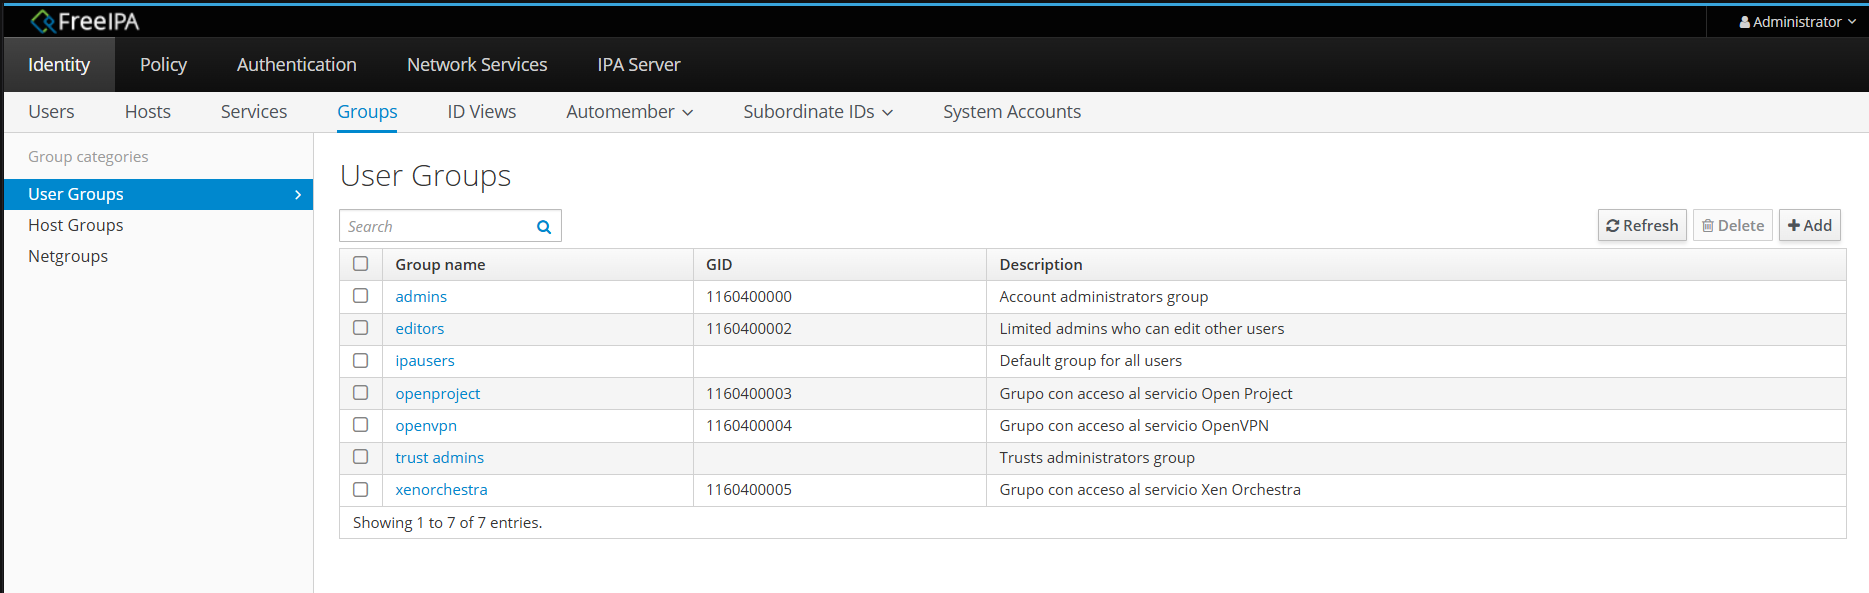
\includegraphics[width=0.8\textwidth]{mainmatter/II-desarrollo-metodologico/implementacion/imagenes/grupos-usuarios.png}
	\caption{Grupos de usuarios configurados en FreeIPA}
	\label{fig:grupos-usuarios}
\end{figure}

\subsection{Políticas de contraseñas}

Una vez creados los grupos de usuarios, se procedió a definir las políticas de contraseñas que regirán el funcionamiento de la plataforma. En primer lugar, se configuró la política global, la cual se aplica de forma predeterminada a todos los usuarios administrados por FreeIPA.

Con el objetivo de fortalecer la seguridad de la infraestructura, se estableció una vigencia máxima de ciento ochenta días para las contraseñas, un período mínimo de veinticuatro horas entre cambios consecutivos y un historial de cinco contraseñas para impedir la reutilización inmediata de credenciales. Asimismo, se definió una longitud mínima de doce caracteres y la obligatoriedad de emplear cuatro categorías de caracteres diferentes.

De igual manera, se limitó a cinco el número máximo de intentos fallidos de autenticación, se configuró un intervalo de sesenta segundos para el restablecimiento del contador de errores y se estableció un período de bloqueo de trescientos segundos. Finalmente, se permitió un máximo de tres inicios de sesión de gracia, los cuales permiten ingresar a los servicios después de vencida la contraseña, esto con el fin de facilitar el cambio de las credenciales una vez alcanzada la fecha de vencimiento. La configuración completa de esta política se presenta en la \autoref{fig:politica-contrasena-global}.

\begin{figure}[H]
	\centering
	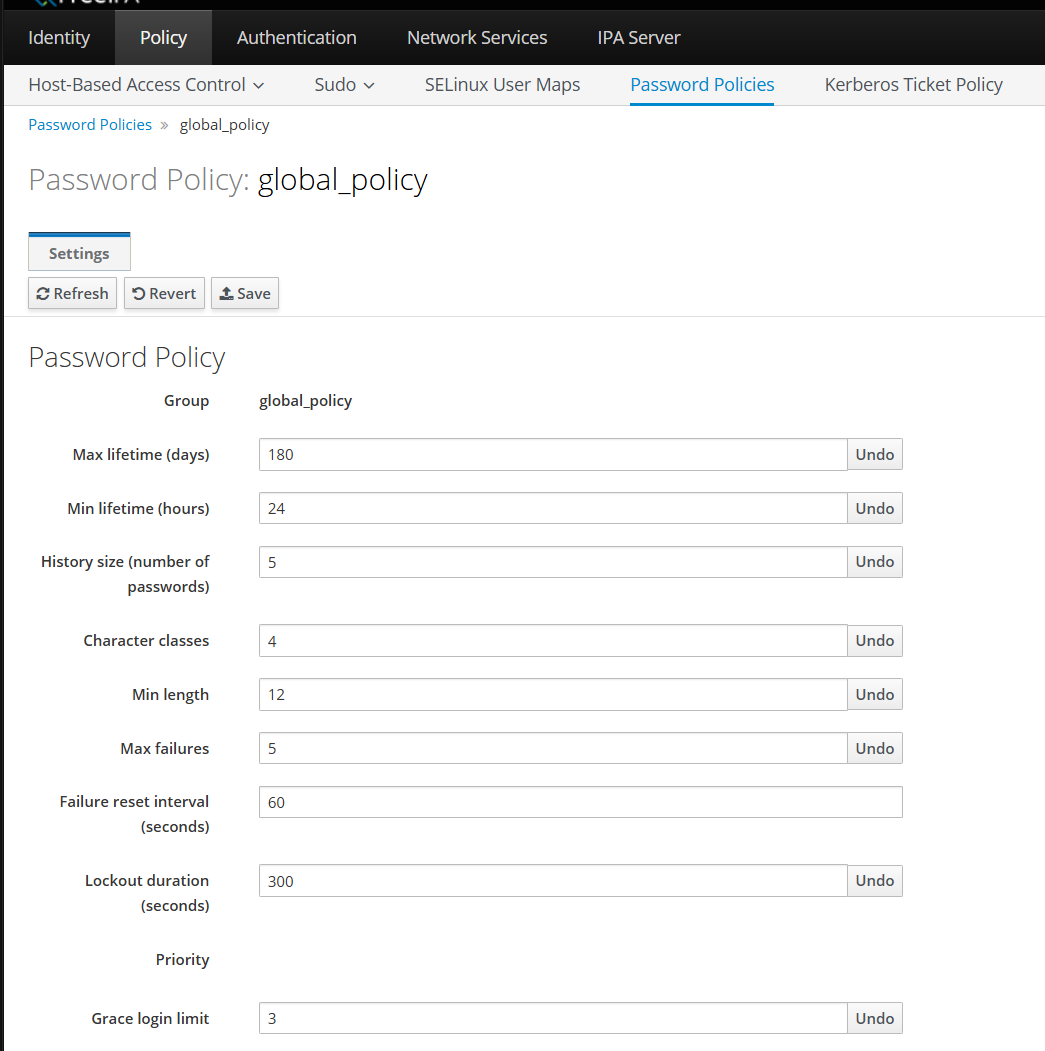
\includegraphics[width=0.8\textwidth]{mainmatter/II-desarrollo-metodologico/implementacion/imagenes/politica-contrasena-global.png}
	\caption{Configuración de la política global de contraseñas}
	\label{fig:politica-contrasena-global}
\end{figure}

Posteriormente, se creó una política específica para el grupo ldap-cuentas-servicio. El propósito de esta configuración fue impedir el vencimiento de las contraseñas asociadas a las cuentas de servicio, garantizando así la disponibilidad continua de los mecanismos de autenticación e integración empleados por las distintas plataformas conectadas al servicio de directorio. La política configurada se observa en la \autoref{fig:politica-contrasena-servicio}.

\begin{figure}[H]
	\centering
	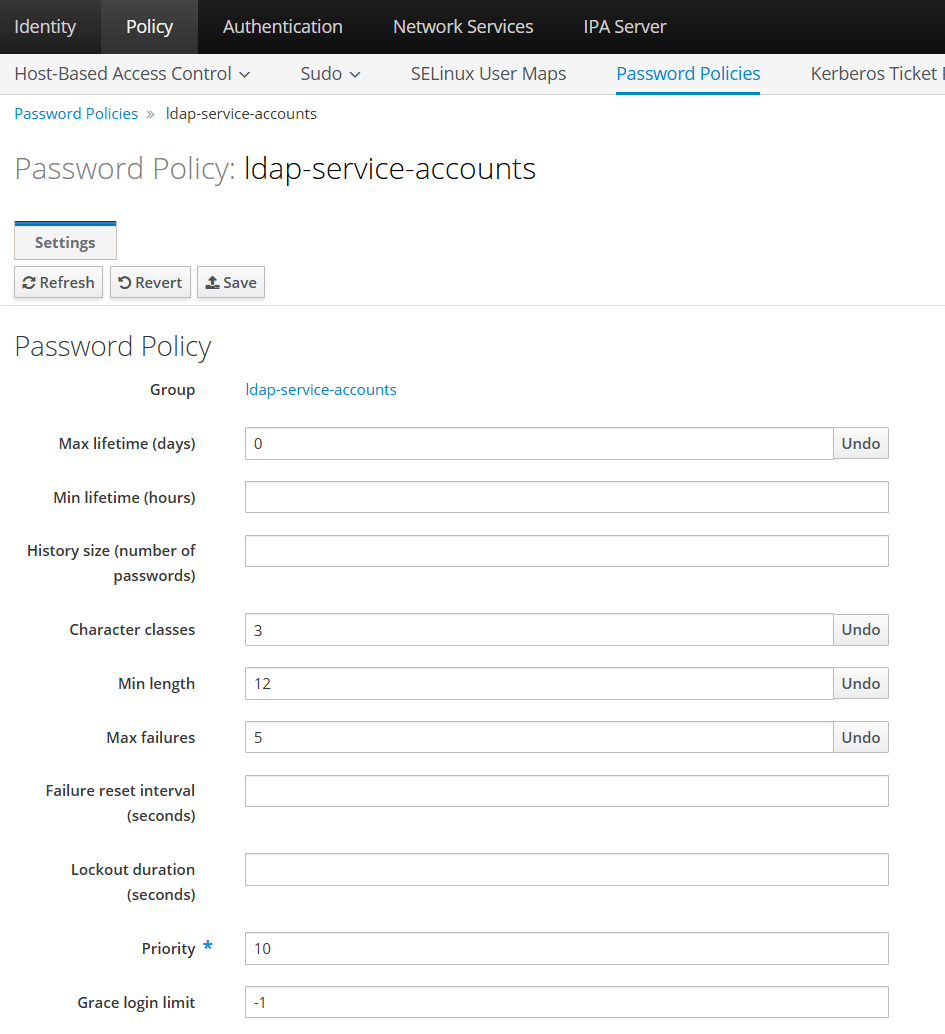
\includegraphics[width=0.8\textwidth]{mainmatter/II-desarrollo-metodologico/implementacion/imagenes/politica-contrasena-servicio.png}
	\caption{Política de contraseñas para las cuentas de servicio}
	\label{fig:politica-contrasena-servicio}
\end{figure}

\subsection{Creación de cuentas de servicio}

Posteriormente, se llevó a cabo la creación de las cuentas de servicio empleadas por las diferentes plataformas para establecer la comunicación con el servidor FreeIPA. Estas cuentas permiten que las aplicaciones realicen consultas al directorio y ejecuten los procesos de autenticación y autorización necesarios para su funcionamiento.

Con el fin de facilitar su administración y aplicar políticas específicas, todas las cuentas creadas fueron incorporadas al grupo ldap-cuentas-servicio. De esta manera, fue posible centralizar la gestión de sus permisos y garantizar la aplicación uniforme de las medidas de seguridad definidas para este tipo de cuentas. Las cuentas de servicio configuradas se presentan en la \autoref{fig:cuentas-servicio}.

\begin{figure}[H]
	\centering
	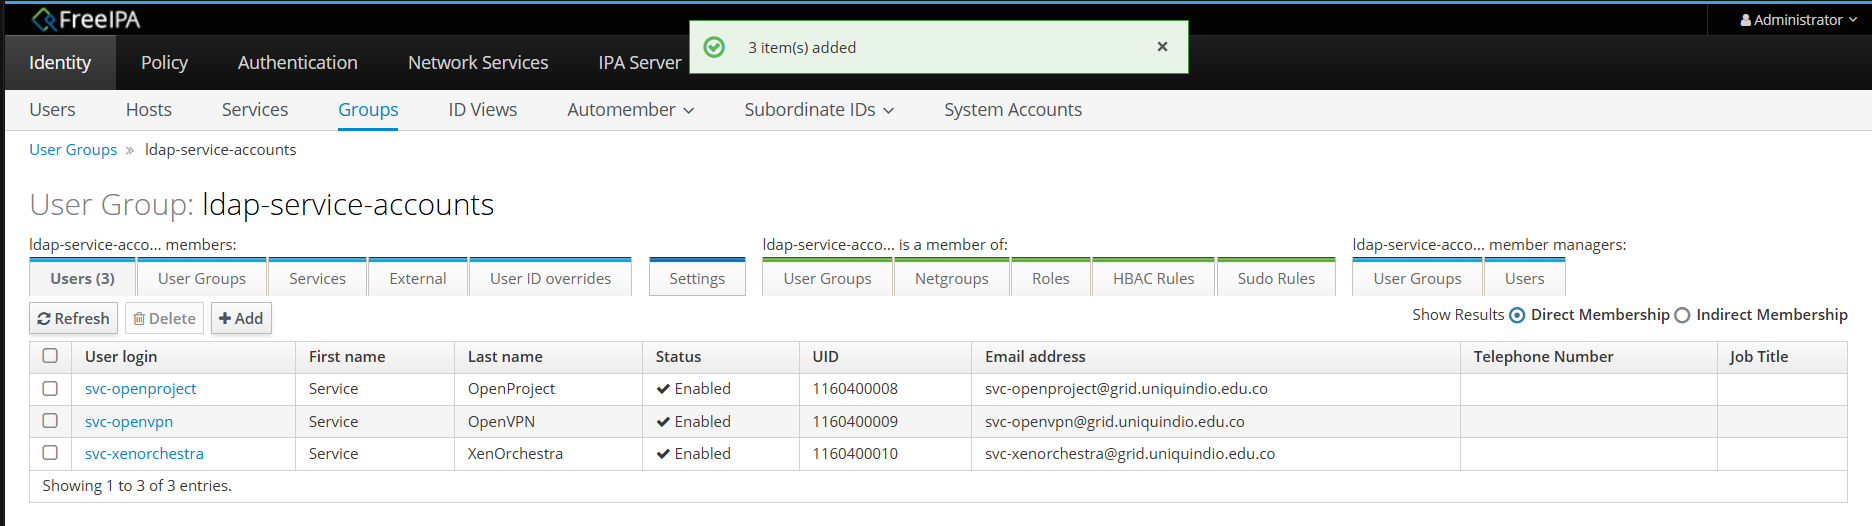
\includegraphics[width=0.8\textwidth]{mainmatter/II-desarrollo-metodologico/implementacion/imagenes/cuentas-servicio.png}
	\caption{Cuentas de servicio configuradas en FreeIPA}
	\label{fig:cuentas-servicio}
\end{figure}

